\documentclass[aps,prb,reprint,superscriptaddress,floatfix]{revtex4-2}

\usepackage{amsmath,amssymb,bm}
\usepackage{graphicx}
\usepackage{hyperref}
\graphicspath{{figures/}}

\newcommand{\FN}{\mathrm{FN}}

\begin{document}

\title{Reconstructing frustrated signs from amplitudes with fixed-node and Krylov updates}

\author{A. Otaifi}
\affiliation{Arnold Sommerfeld Center for Theoretical Physics, Ludwig-Maximilians-Universit\"at M\"unchen, 80333 M\"unchen, Germany}
\date{\today}

\begin{abstract}
We separate the sign and positive-amplitude parts of a real many-body wave
function, $\psi(x)=s(x)a(x)$ with $a(x)=|\psi(x)|>0$, in the frustrated
square-lattice spin-$1/2$ $J_1$--$J_2$ Heisenberg model. For a fixed
amplitude, one shifted Krylov step gives
$s'(x)=s(x)\operatorname{sgn}[T-r_s(x)]$, where
$r_s(x)=(H\psi)(x)/\psi(x)$. At $J_2/J_1=0.5$ this reduces the exact
$4\times4$ probability weight on incorrectly signed configurations from
$1.27\times10^{-2}$ to $3.41\times10^{-4}$. On $6\times6$, using exactly
the same neural-network amplitude, the reconstructed signs give the same
energy as the original neural-network signs within sampling uncertainty.
Conversely, lattice fixed-node projection improves the positive amplitude
while keeping the signs fixed; an exact $4\times4$ fixed-node/Krylov loop
reaches the exact ground-state signs. The reconstructed signs remain useful
on $8\times8$. The remaining scaling problem is to infer from fixed-node
Monte Carlo walkers a positive amplitude function that can be evaluated on
arbitrary configurations. Maximum likelihood targets
$a_{\rm new}^2\propto a\phi_{\FN}$, and stochastic reconfiguration produces
an update that generalizes between independent walker samples.
\end{abstract}

\maketitle

\section{Introduction}

The Monte Carlo sign problem is severe in frustrated spin systems
\cite{HeneliusSandvik2000,TroyerWiese2005}. We use the square-lattice
$J_1$--$J_2$ Heisenberg model as a benchmark. At $J_2=0$ its ground-state
signs obey the Marshall rule \cite{Marshall1955}; near $J_2/J_1=1/2$ that
rule fails and accurate variational states become nontrivial
\cite{Choo2019,ChenHeyl2024}.

We ask whether signs and positive amplitudes can be improved separately.
For a real wave function we write
\begin{equation}
\psi(x)=s(x)a(x),\qquad s(x)=\pm1,\quad a(x)=|\psi(x)|>0 .
\label{eq:decomp}
\end{equation}
Given $a$, a single Krylov step updates the signs. Given $s$, lattice fixed
node gives a sign-free positive-amplitude problem \cite{vanBemmel1994}.
Our calculations first test these two operations separately and then close
the feedback loop.

\section{Model and method}

We study
\begin{equation}
H=J_1\sum_{\langle ij\rangle}\mathbf S_i\!\cdot\!\mathbf S_j
 +J_2\sum_{\langle\!\langle ij\rangle\!\rangle}
 \mathbf S_i\!\cdot\!\mathbf S_j ,
\label{eq:H}
\end{equation}
on periodic $L\times L$ lattices with $J_1=1$ in the $S^z=0$ sector.
For a spin configuration $x$, the Marshall rule is
$s_M(x)=(-1)^{N^A_\downarrow(x)}$ up to an overall sign, where
$N^A_\downarrow$ counts down spins on one checkerboard sublattice.

\subsection{One-step sign update}

For $\psi=sa$, define the local energy
\begin{equation}
r_s(x)=\frac{(H\psi)(x)}{\psi(x)} .
\label{eq:localenergy}
\end{equation}
Because
\begin{equation}
[(T-H)\psi](x)=[T-r_s(x)]\psi(x),
\end{equation}
the sign of the shifted Krylov vector is
\begin{equation}
s_{\rm K}(x)=s(x)\operatorname{sgn}[T-r_s(x)] .
\label{eq:k1}
\end{equation}
Only this sign is kept; the Krylov amplitude factor $|T-r_s(x)|$ is
discarded. Thus the method is not repeated Lanczos multiplication. For exact
systems, $T$ is chosen to minimize the fixed-amplitude variational energy.
For sampled systems, $T$ is obtained from a two-cluster split of the
$r_s(x)$ values and therefore does not use target sign labels.

When the exact ground state $\psi_0=s_0a_0$ is available, we fix the
irrelevant overall sign and report directly the wrong-sign probability
weight
\begin{equation}
w_s=\sum_{x:\,s(x)\neq s_0(x)} a_0(x)^2 .
\label{eq:signweight}
\end{equation}

\subsection{Fixed-node amplitude update}

For a trial wave function $\psi_T$, an off-diagonal matrix element connecting
$x$ and $y$ is sign violating when
$H_{xy}\psi_T(y)/\psi_T(x)>0$. Lattice fixed node removes such off-diagonal
terms and adds their contribution to the diagonal \cite{vanBemmel1994}.
After importance sampling, the resulting Hamiltonian is sign free and keeps
the signs of $\psi_T$ fixed.

Let $\phi_{\FN}(x)>0$ be the positive ground-state amplitude obtained from
this fixed-node Hamiltonian. In an exact small-system calculation,
$\phi_{\FN}$ can be inserted directly into Eq.~\eqref{eq:k1}. In a walker
calculation, however, the stationary sampled distribution is
\begin{equation}
f(x)\propto a(x)\phi_{\FN}(x) .
\label{eq:mixed}
\end{equation}
If a positive model is trained by maximum likelihood with
$p_\theta(x)\propto a_\theta(x)^2$, the exact maximum-likelihood target is
\begin{equation}
a_{\rm new}^2(x)\propto a(x)\phi_{\FN}(x) .
\label{eq:halfstep}
\end{equation}
Since $a_{\rm new}(x)>0$, this is equivalent to taking the geometric mean of
the current and fixed-node amplitudes.

The $4\times4$ exact calculations use the full $S^z=0$ Hilbert space of
$12\,870$ states. For $6\times6$ and $8\times8$ we use a previously optimized
translationally invariant vision-transformer neural quantum state (ViT) at
$J_2/J_1=0.5$. In the sign-only benchmarks, its positive amplitude
$|\psi_{\rm ViT}(x)|$ is held fixed. The $8\times8$ fixed-node calculations
use a walker population $M=128$ and projection length $\beta=1.2$.

\begin{figure*}[t]
\centering
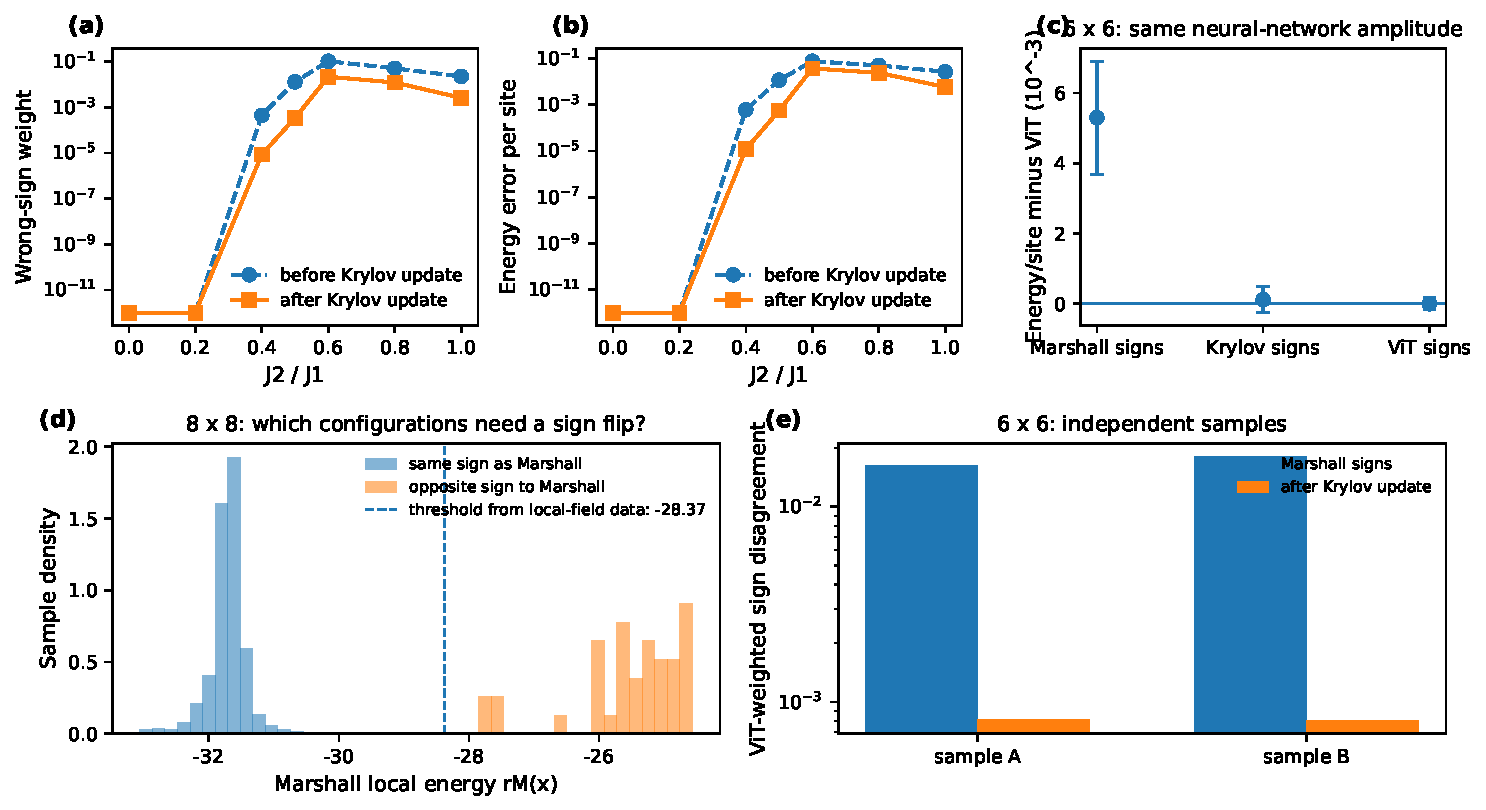
\includegraphics[width=0.98\textwidth]{fig2_sign_story.pdf}
\caption{Sign reconstruction. (a,b) Exact $4\times4$ wrong-sign weight
$w_s$ and fixed-amplitude energy error. The initial sign rule is Marshall for
$J_2/J_1\leq0.6$ and a stripe rule for $J_2/J_1\geq0.8$; the stripe rule
uses alternating columns instead of the checkerboard sublattices of the
Marshall rule. The positive amplitude is always the exact ground-state
amplitude. (c) $6\times6$ energies obtained with the same ViT positive
amplitude and three different sign patterns; error bars are between-chain
standard errors. (d) $8\times8$ distributions of the Marshall local energy
$r_M(x)$. ViT signs are used only afterward to identify configurations that
agree or disagree with Marshall; the threshold is obtained from the $r_M$
values alone. (e) Fraction of the ViT probability weight
$|\psi_{\rm ViT}|^2$ whose sign disagrees with the ViT sign, before and
after the Krylov update, on two independent samples. Exact zeros in
panels (a,b) are displayed at $10^{-12}$ only to make them visible on the
logarithmic axes.}
\label{fig:signbench}
\end{figure*}

\section{One-step sign reconstruction}

Figure~\ref{fig:signbench}(a,b) uses the exact $4\times4$ positive
ground-state amplitude. At $J_2/J_1=0.5$, Marshall signs place
$1.27\times10^{-2}$ of the exact ground-state probability on configurations
with the wrong sign. One Krylov update reduces this to
$3.41\times10^{-4}$ and lowers the fixed-amplitude energy error per site from
$1.16\times10^{-2}$ to $5.51\times10^{-4}$.

The $6\times6$ test no longer uses exact signs. With the same ViT positive
amplitude for all three states,
\begin{align}
e_{\rm Marshall}&=-0.4981534,\nonumber\\
e_{\rm Krylov}&=-0.5033337,\nonumber\\
e_{\rm ViT}&=-0.5034504 .
\end{align}
The paired difference
$e_{\rm Krylov}-e_{\rm ViT}=1.17(287)\times10^{-4}$ is unresolved, whereas
Krylov improves over Marshall by $4.79\times10^{-3}$ per site. The energy
gain therefore comes from the signs, not from changing the amplitude.

The mechanism is visible in the Marshall local energy,
\begin{equation}
r_M(x)=D(x)+F_{J_1}(x)+F_{J_2}(x),
\end{equation}
where $D$ is the diagonal contribution and $F_{J_1},F_{J_2}$ are the two
off-diagonal exchange contributions. The useful signal is mainly their
competition. On two independent $6\times6$ samples, the fraction of
$|\psi_{\rm ViT}|^2$ weight with the wrong sign falls from $0.01635$ to
$8.08\times10^{-4}$ and from $0.01811$ to $8.02\times10^{-4}$,
respectively.

\begin{figure*}[t]
\centering
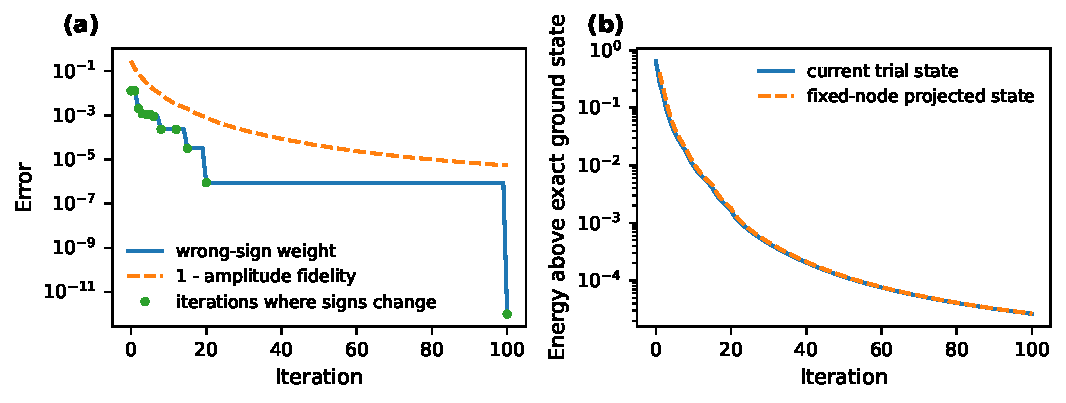
\includegraphics[width=0.82\textwidth]{fig3_closed_loop.pdf}
\caption{Exact $4\times4$ fixed-node/Krylov loop at $J_2/J_1=0.5$.
(a) Wrong-sign weight $w_s$ and amplitude error $1-F_a$. For normalized
positive amplitudes, $F_a=|\langle a|a_0\rangle|^2$. Markers indicate
iterations at which the sign pattern changes. The exact zero reached at
the end is displayed at $10^{-12}$ on the logarithmic axis. (b) Energy above
the exact ground state for the current trial state and for the fixed-node
projected state.}
\label{fig:closedloop}
\end{figure*}

\section{Closing the loop exactly}

We target $J_2/J_1=0.5$ but initialize with the exact positive ground-state
amplitude at $J_2=0$ and Marshall signs. At each iteration we solve the
current fixed-node problem exactly, replace the positive amplitude by the
fixed-node ground-state amplitude, and recompute Eq.~\eqref{eq:k1}. The exact
$J_2/J_1=0.5$ ground state is used only to evaluate the plotted errors.

Initially $F_a=0.7132$ and the wrong-sign weight is $w_s=1.27\times10^{-2}$.
After two iterations $w_s=2.03\times10^{-3}$; after twenty,
$w_s=8.85\times10^{-7}$; at iteration 100 it is zero to numerical precision.
The final amplitude fidelity is $0.9999946$, and the energy of the current
trial state is $2.60\times10^{-5}$ above the exact ground state.

The plateaus in Fig.~\ref{fig:closedloop}(a) have a simple interpretation:
fixed node can improve the amplitude for several iterations without changing
any sign. A new sign pattern appears only when the improved amplitude moves
the local-energy threshold across additional configurations.

\begin{figure*}[t]
\centering
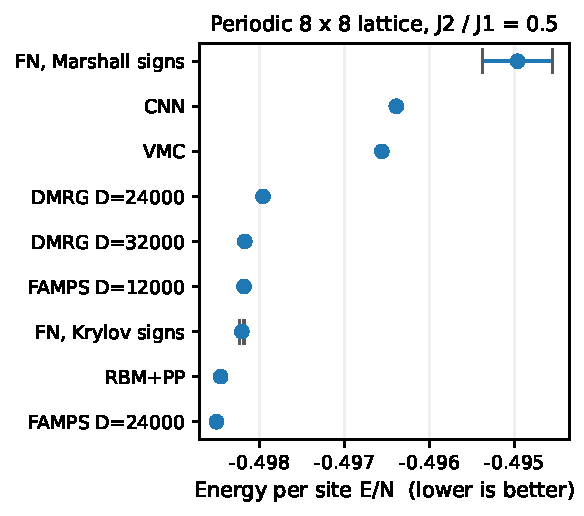
\includegraphics[width=0.55\textwidth]{fig4_8x8_benchmark.pdf}
\caption{Energy per site on the periodic $8\times8$ lattice at
$J_2/J_1=0.5$. ``FN'' denotes lattice fixed node. The two FN entries use
Marshall signs or the one-step Krylov-reconstructed signs. Short ticks show
the two independent walker populations. Literature values are from
Ref.~\cite{QianQin2023}.}
\label{fig:8x8bench}
\end{figure*}

\section{Scaling to $8\times8$}

At $M=128$, the mean total fixed-node energies from two independent walker
populations are
\begin{equation}
E_{\rm Krylov}=-31.88542,\qquad
E_{\rm Marshall}=-31.67748 .
\end{equation}
Their difference is $-0.20795$. With only two populations, their spread is
used only as a reproducibility scale.

Using the Krylov-reconstructed signs gives $E/N=-0.498210$, compared with
$-0.494961$ when the same fixed-node calculation uses Marshall signs.
Figure~\ref{fig:8x8bench} shows that it lies in the same energy range as
high-accuracy DMRG/FAMPS and neural benchmarks on the same geometry. We use
this only as a scale comparison, not as a ranking between methods.

Thus the reconstructed signs remain useful on $8\times8$. The remaining
problem is to infer from fixed-node walkers a positive amplitude function
that can be evaluated on configurations not present in the walker sample.

\begin{figure*}[t]
\centering
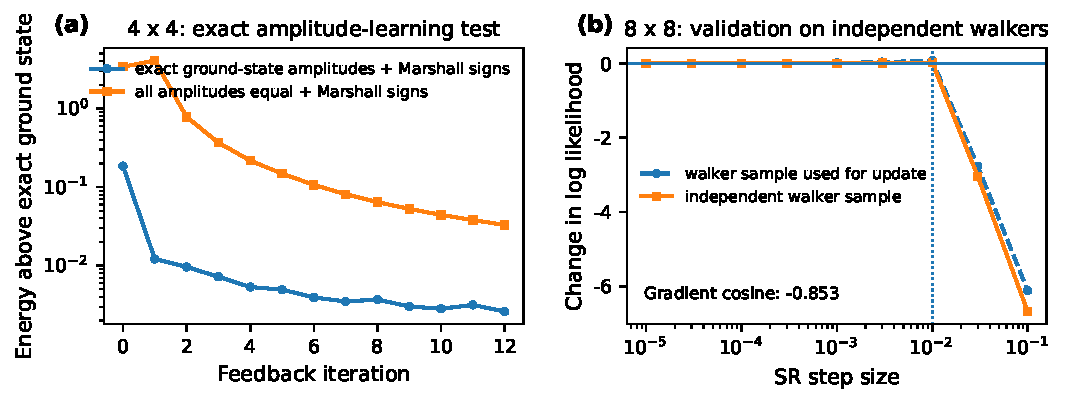
\includegraphics[width=0.82\textwidth]{fig5_amplitude_learning.pdf}
\caption{Learning the positive amplitude. (a) Exact $4\times4$ test of
Eq.~\eqref{eq:halfstep}. ``Exact amplitudes'' means the exact
$J_2/J_1=0.5$ ground-state amplitudes; ``equal amplitudes'' means the same positive value $a(x)=\mathrm{const.}$
for every basis state, followed by normalization. Both start with
Marshall signs. (b) Stochastic-reconfiguration (SR) step-size scan on
$8\times8$: the update is fitted to one fixed-node walker sample and evaluated
on an independent sample.}
\label{fig:amplearn}
\end{figure*}

\section{Learning the amplitude from walkers}

Equation~\eqref{eq:halfstep} can be tested exactly on $4\times4$. Starting
from the exact $J_2/J_1=0.5$ ground-state amplitudes but assigning Marshall
signs, one exact amplitude update from Eq.~\eqref{eq:halfstep} followed by
the Krylov sign update changes the energy from $-8.27291$ to $-8.44579$,
close to $E_0=-8.45792$. A deliberately poor start in which all positive
amplitudes are equal initially moves to higher energy, but later iterations
recover [Fig.~\ref{fig:amplearn}(a)].

At $8\times8$, let $g_1$ and $g_2$ be maximum-likelihood gradients estimated
from two independent fixed-node walker samples. Their Euclidean cosine is
\begin{equation}
\frac{g_1\cdot g_2}{\|g_1\|\,\|g_2\|}=-0.853,
\end{equation}
so an ordinary gradient step fitted to one sample does not generalize to the
other.

We therefore use stochastic reconfiguration (SR) \cite{Sorella2001},
\begin{equation}
\delta\theta=(S+\lambda I)^{-1}g_1 ,
\end{equation}
where $S$ is the empirical Fisher matrix of the amplitude model and
$\lambda$ is a diagonal regularization.
For $\lambda=1$, the directional derivative on the independent second walker
sample becomes $g_2^{\mathsf T}\delta\theta=+3.85$. The finite step-size scan
in Fig.~\ref{fig:amplearn}(b) remains positive and peaks near $\eta=0.01$,
where the log-likelihood change on the independent sample is $+0.0156$ and
the reweighting effective sample size is $3236/4096$.

This shows that one learned amplitude update generalizes between independent
walker samples. It does not yet establish convergence of repeated
$8\times8$ updates; the fixed-node energy remains the acceptance test.

\section{Discussion and outlook}

The data separate the two tasks. With a good positive amplitude, the dominant
frustrated sign correction is captured by a threshold in the local energy.
Fixed node solves the complementary positive-amplitude problem at fixed signs,
and the exact $4\times4$ loop shows that the two updates can close.

The unresolved large-system problem is learning that positive amplitude from
projector walkers. SR makes one $8\times8$ update generalize between
independent walker samples, but repeated updates still require fixed-node
energy validation. The method also requires a useful initial amplitude and
should not be confused with repeated bare Krylov iteration; the direct second
step is worse on $6\times6$.

\appendix

\section{Direct second Krylov step}

On $6\times6$, retaining the full first Krylov amplitude gives
$a_1(x)=|T_1-r_0(x)|a_0(x)$ with coefficient of variation about $0.18$.
A second unsupervised threshold changes only $0.8$--$2.0\%$ of the
$|\psi_{\rm ViT}|^2$ probability weight but raises the fixed-amplitude energy
by $0.65$--$0.96$ in total energy. The feedback construction therefore
restores or re-solves the amplitude before another sign update.

\section{Statistical convention}

Exact-diagonalization data are deterministic up to eigensolver precision.
For the $6\times6$ fixed-amplitude comparison we use correlation-robust
between-chain standard errors. For $8\times8$ fixed-node data with two
independent walker populations, error bars denote half the population
difference and are treated only as reproducibility scales.

\bibliography{refs}
\end{document}
